% Appendix A

\chapter{Implementatie en resultaten} % Main appendix title

\label{BijlageCode} 

\section{Docker-compose opstelling voor k6, InfluxDB \& Grafana}

\label{Bijlagek6}

Om de loadtest met k6, influxDB en grafana op te stellen heeft Loadimpact een docker-compose opstelling gemaakt. Na wat onderzoek is het opgevallen dat deze opstelling erg verouderd is. Daarom is ervoor gekozen om een eigen opstelling te maken:
\begin{minted}[linenos=true, bgcolor=codebg, breaklines]{yaml}
version: '3.4'

networks:
  k6:
  grafana:

services:
  influxdb:
    image: influxdb:1.5.4
    networks:
    - k6
    - grafana
    ports:
      - "8086:8086"
    environment:
      - INFLUXDB_DB=k6
    
  grafana:
    image: grafana/grafana:6.4.1
    networks:
      - grafana
    ports:
      - "3000:3000"
    environment:
      - GF_AUTH_ANONYMOUS_ORG_ROLE=Admin
      - GF_AUTH_ANONYMOUS_ENABLED=true
      - GF_AUTH_BASIC_ENABLED=false
    volumes:
      - ./grafana/datasource.yml:/etc/grafana/provisioning/datasources /datasource.yml
  
  k6:
    image: loadimpact/k6:0.25.1
    networks:
      - k6
    ports:
      - "6565:6565"
    environment:
      - K6_OUT=influxdb=http://influxdb:8086/k6
    volumes:
      - ../k6:/k6
\end{minted}

Hiervoor is een Pull-Request gemaakt naar loadimpact/k6 om dit te verbeteren. \texttt{https://github.com/loadimpact/k6/pull/1183} samen met de issue\\ \texttt{https://github.com/loadimpact/k6/issues/1182}. Hierin is te lezen wat precies de veranderingen waren. De maintainers van k6 waren blij met de verandering en hebben deze geaccepteerd en gemerged naar master. De loadtest is geschreven in javascript met de volgende code:
\begin{minted}[linenos=true, bgcolor=codebg, breaklines]{javascript}
import http from "k6/http";
import { sleep, check } from "k6";

export let options = {
  stages: [
    { duration: "10s", target: 20 },
    { duration: "10s", target: 40 },
    { duration: "10s", target: 60 },
    { duration: "10s", target: 80 },
    { duration: "10s", target: 100 },
    { duration: "10s", target: 120 },
  ]
};

export default function() {
  check(http.get("https://test.developers.nl/"), {
    "is status 200": (r) => r.status === 200
  });
  sleep(1);
};
\end{minted}

\section{k6 load test resultaten}

\label{bijlageloadtest}

In figuur \ref{fig:loadtestcli} is de CLI output van de loadtest te vinden. In figuur \ref{fig:loadtestvus} zijn de oplopende hoeveelheid VUs uitgebeeld in Grafana, en in figuur \ref{fig:loadtestresultaten} is in Grafana te zien hoe lang de requests duren.
\begin{figure}[H]
	\centering
	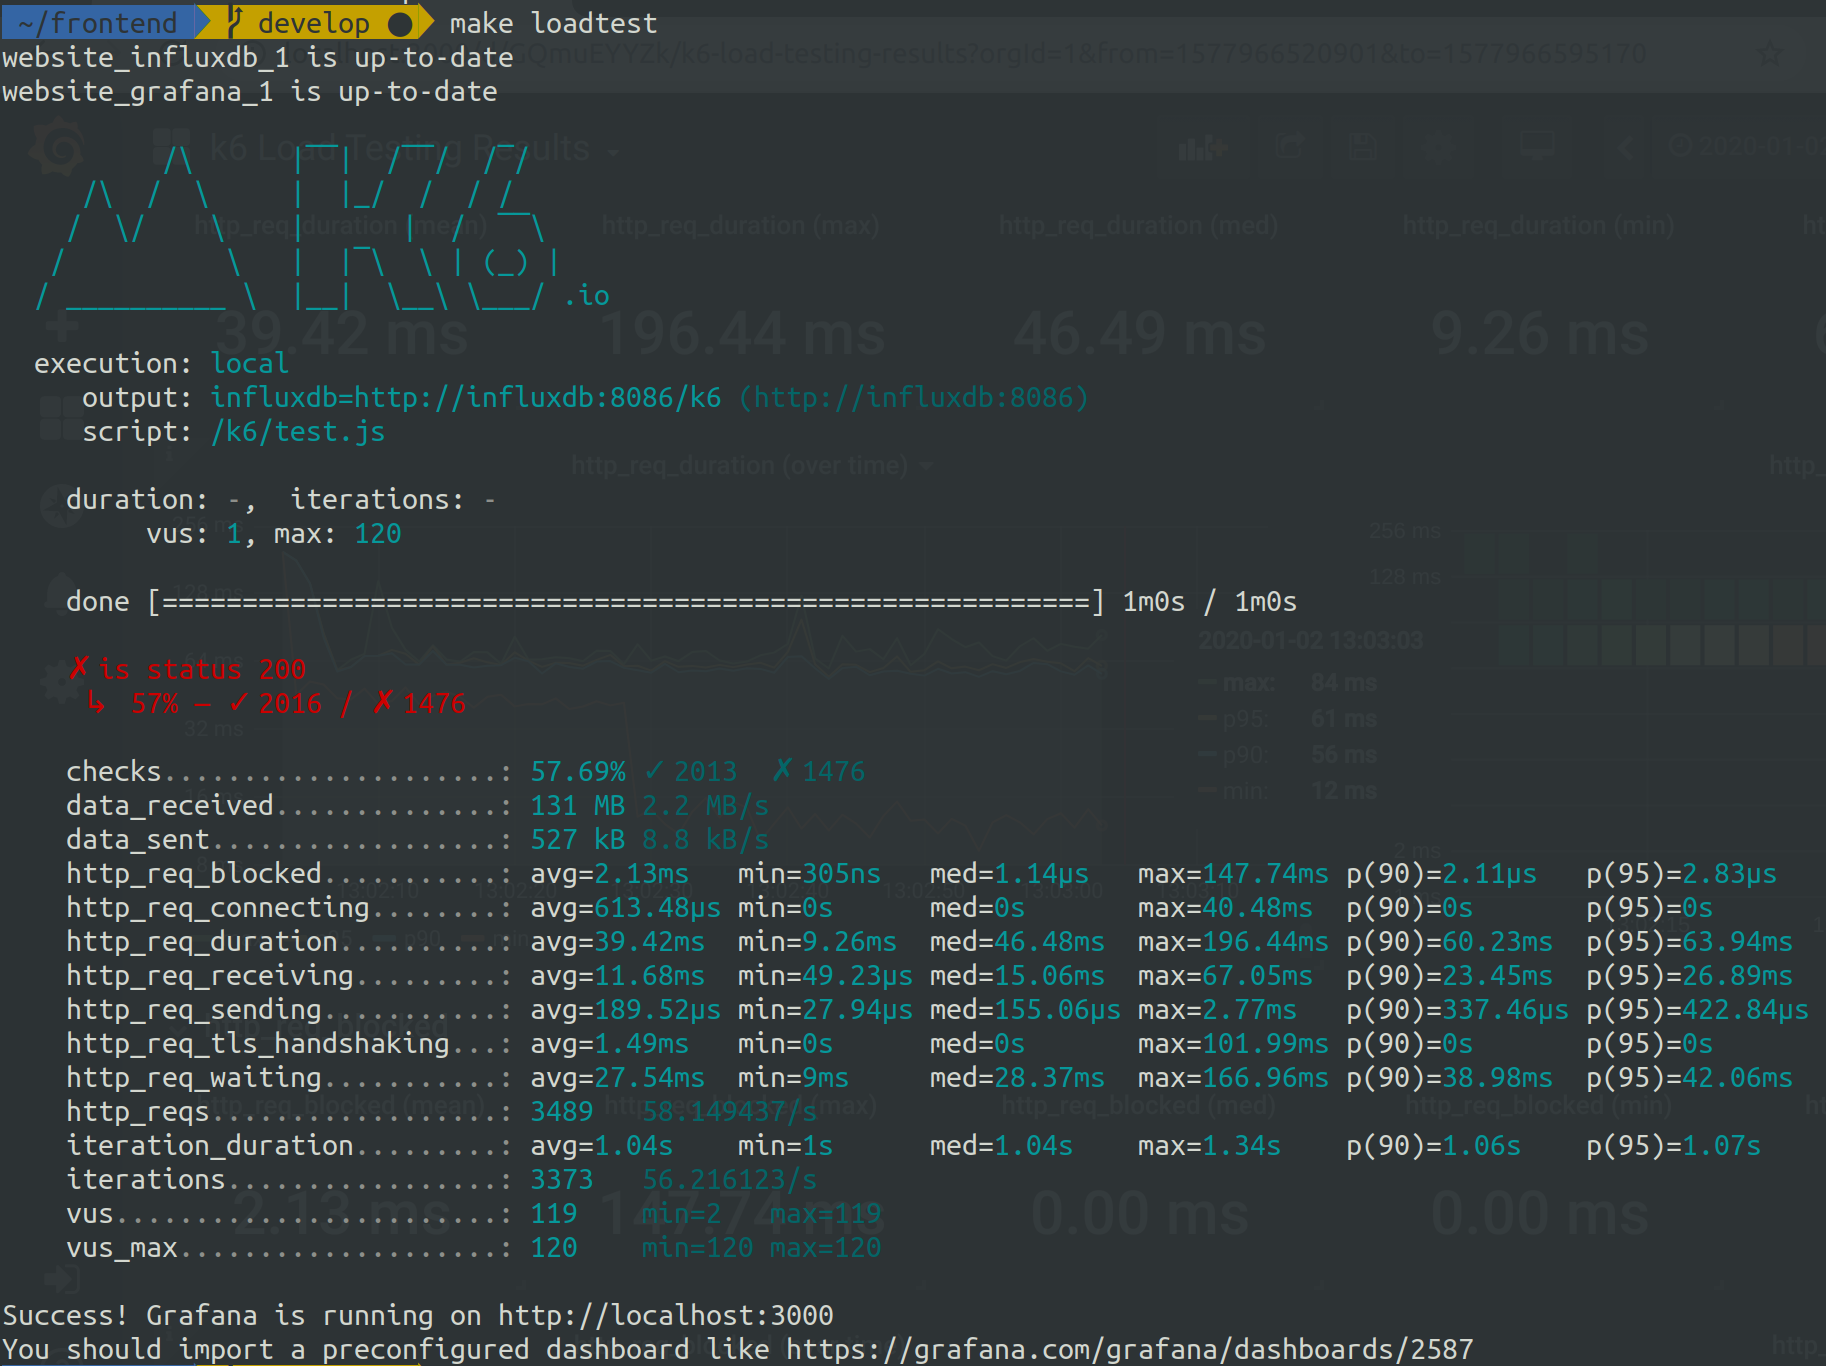
\includegraphics[width=13cm]{Figures/loadtest}
	\decoRule
	\caption[k6 loadtest CLI resultaten]{k6 loadtest CLI resultaten}
	\label{fig:loadtestcli}
\end{figure}

\begin{figure}[H]
	\centering
	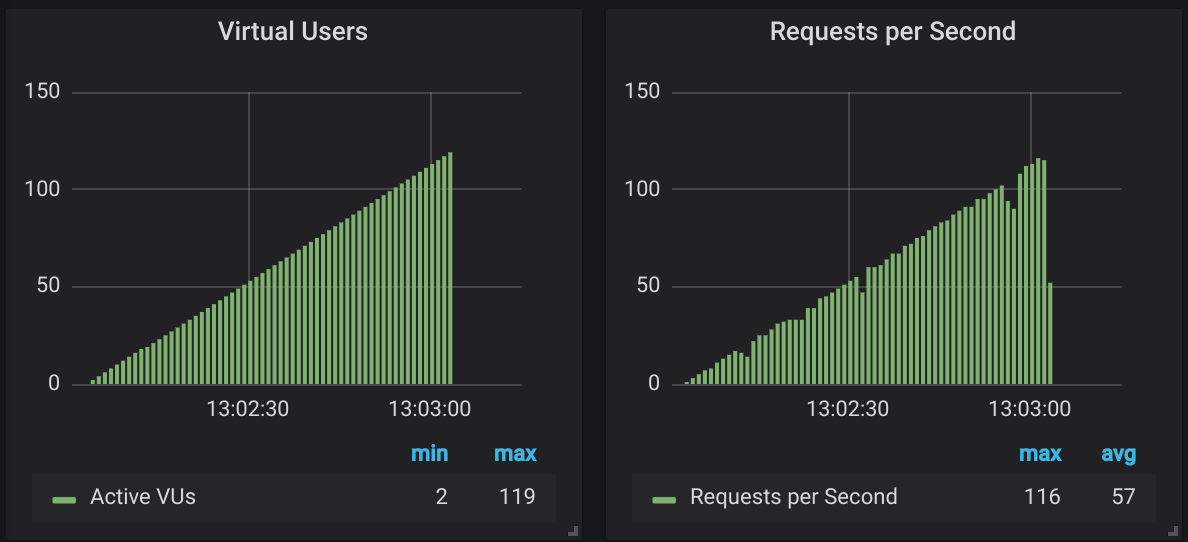
\includegraphics[width=13cm]{Figures/loadtestusers}
	\decoRule
	\caption[k6 loadtest hoeveelheid VUs en requests]{k6 loadtest hoeveelheid VUs en requests}
	\label{fig:loadtestvus}
\end{figure}

\begin{figure}[H]
	\centering
	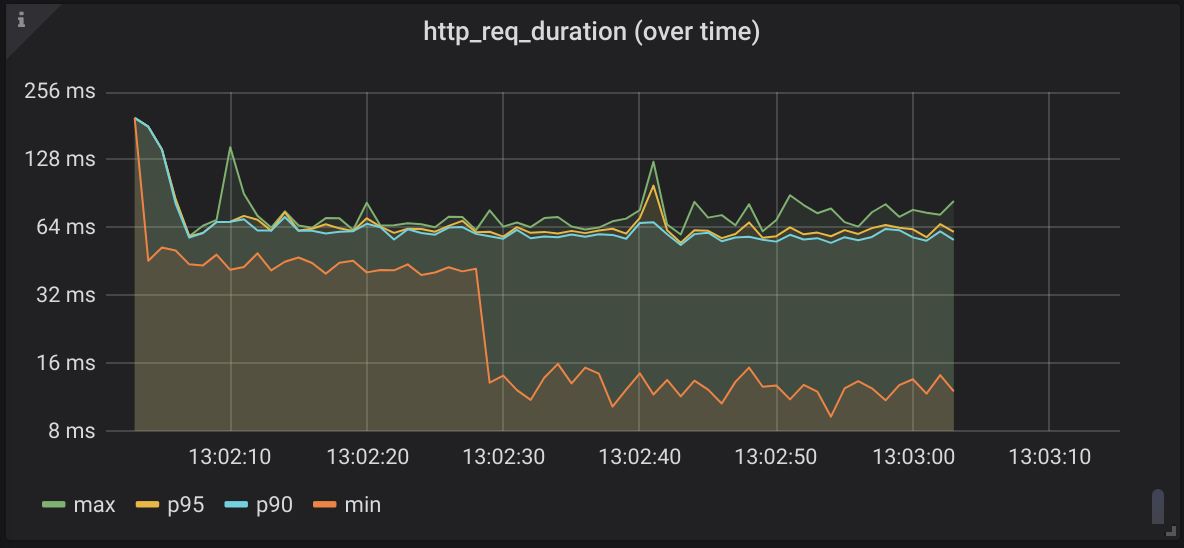
\includegraphics[width=13cm]{Figures/loadtestrequests}
	\decoRule
	\caption[k6 loadtest resultaten]{k6 loadtest resultaten}
	\label{fig:loadtestresultaten}
\end{figure}


\section{Docker container exits}

\label{DockerExits}

\subsubsection{PostgreSQL}
\begin{minted}[linenos=true, bgcolor=codebg, breaklines]{text}
LOG: received smart shutdown request
LOG: background worker "logical replication launcher" (PID 43) exited with exit code 1
LOG: shutting down
LOG: database system is shut down
\end{minted}

\subsubsection{PHP-FPM}
\begin{minted}[linenos=true, bgcolor=codebg, breaklines]{text}
NOTICE: Terminating ...
NOTICE: exiting, bye-bye!
\end{minted}

\subsubsection{Redis}
\begin{minted}[linenos=true, bgcolor=codebg, breaklines]{text}
1:signal-handler (1570781278) Received SIGTERM scheduling shutdown...
# User requested shutdown...
* Saving the final RDB snapshot before exiting.
* DB saved on disk
* Removing the pid file.
# Redis is now ready to exit, bye bye...
\end{minted}

\subsubsection{Nginx}
\begin{minted}[linenos=true, bgcolor=codebg, breaklines]{text}
[notice] 1#1: signal 15 (SIGTERM) received from 56, exiting
[notice] 48#48: exiting
[notice] 47#47: exiting
[notice] 47#47: exit
[notice] 1#1: signal 14 (SIGALRM) received
[notice] 1#1: signal 17 (SIGCHLD) received from 48
[notice] 1#1: cache manager process 48 exited with code 0
[notice] 1#1: worker process 47 exited with code 0
[notice] 1#1: exit
\end{minted}

\section{Docker container kill \& restarts}

\label{DockerKills}

\begin{minted}[linenos=true, bgcolor=codebg, breaklines]{text}
$ docker ps -q
d0829783af18
f72e9967771b
01dd48ff5a59
fab794731d47
ca510c065d11
3ee85578efb5

$ docker kill $(docker ps -q) 

$ docker ps
d0829783af18
f72e9967771b
01dd48ff5a59
fab794731d47
ca510c065d11
3ee85578efb5

$ docker ps -q

$ docker start $(docker ps -aq)
d0829783af18
f72e9967771b
01dd48ff5a59
fab794731d47
d68d7ab9809c
ca510c065d11
3ee85578efb5
e1866ab6c1af

$ docker ps -q
d0829783af18
f72e9967771b
01dd48ff5a59
fab794731d47
ca510c065d11
3ee85578efb5
\end{minted}

\section{Codecov implementatie} \label{codecov}
README.MD:
\begin{minted}[linenos=true, bgcolor=codebg, breaklines]{text}
## Tests

We enforce that code coverage stays acceptable using codecov:

[![codecov](https://codecov.io/bb/developers_nl/developers.nl/branch/ma
ster/graph/badge.svg?token=DzAv79t9Gd)](https://codecov.io/bb/developer
s_nl/developers.nl)
\end{minted}

Het builden van de Docker images met Ansible, inclusief de build arguments nodig voor codecov:
\begin{minted}[linenos=true, bgcolor=codebg, breaklines]{yaml}
docker_images:
  - dockerfile: docker/php7-fpm/Dockerfile
  path: ../
  name: developersnl/website-php-fpm
  buildargs:
    GROUP_ID: 9000
    USER_ID: 9000
    BITBUCKET_BRANCH: "{{ lookup('env','BITBUCKET_BRANCH') }}"
    BITBUCKET_COMMIT: "{{ lookup('env', 'BITBUCKET_COMMIT') }}"
    BITBUCKET_BUILD_NUMBER: "{{ lookup('env','BITBUCKET_BUILD_NUMBER') }}"
    BITBUCKET_REPO_OWNER: "{{ lookup('env','BITBUCKET_REPO_OWNER') }}"
    BITBUCKET_REPO_SLUG: "{{ lookup('env','BITBUCKET_REPO_SLUG') }}"
    BITBUCKET_PR_ID: "{{ lookup('env','BITBUCKET_PR_ID') }}"
    CODECOV_TOKEN: "{{ lookup('env','CODECOV_TOKEN') }}"
    CI: "{{ lookup('env','CI') }}"
\end{minted}

In de php7-fpm dockerfile zijn de build args omgezet naar environment variablen, een aantal apk packages toegevoegd en is het codecov script toegevoegd:
\begin{minted}[linenos=true, bgcolor=codebg, breaklines]{bash}
FROM application AS test

ENV SYMFONY_PHPUNIT_VERSION 8.0.0

ARG BITBUCKET_BRANCH
ARG BITBUCKET_BUILD_NUMBER
ARG BITBUCKET_REPO_OWNER
ARG BITBUCKET_REPO_SLUG
ARG BITBUCKET_PR_ID
ARG CODECOV_TOKEN
ARG CI
ARG BITBUCKET_COMMIT

ENV BITBUCKET_BRANCH=$BITBUCKET_BRANCH
ENV BITBUCKET_BUILD_NUMBER=$BITBUCKET_BUILD_NUMBER
ENV BITBUCKET_REPO_OWNER=$BITBUCKET_REPO_OWNER
ENV BITBUCKET_REPO_SLUG=$BITBUCKET_REPO_SLUG
ENV BITBUCKET_PR_ID=$BITBUCKET_PR_ID
ENV CODECOV_TOKEN=$CODECOV_TOKEN
ENV CI=$CI

# TODO: Cange VCS_COMMIT_ID to BITBUCKET_COMMIT when https://github.com/codecov/codecov-bash/pull/225 is deployed
ENV VCS_COMMIT_ID=$BITBUCKET_COMMIT

COPY --from=composer:1.9.0 /usr/bin/composer /usr/bin/composer

RUN apk add \
    php7-pdo_sqlite \
    php7-sqlite3 \
    php7-phar \
    php7-pear \
    php7-dev \
    redis \
    curl \
    bash \
    git \
    mercurial \
    findutils \
    g++ \
    make \
 && . /bin/pcov.sh \
 && redis-server --daemonize yes --requirepass test \
 && composer install -d /app/src --optimize-autoloader --no-interaction --no-suggest --no-scripts \
 && chmod u+x,g+x /app/src/bin/phpunit \
 && /app/src/bin/phpunit --configuration /app/src/phpunit.xml --coverage-clover=coverage.xml \
 && curl -s https://codecov.io/bash | bash -s - -X coveragepy
\end{minted}

pcov script:
\begin{minted}[linenos=true, bgcolor=codebg, breaklines]{bash}
#!/bin/sh

# Add PHP Coverage ini configuration
echo "- Enabling pcov"
cat <<-EOF > /etc/php7/conf.d/pcov.ini
extension=pcov
pcov.enable=1
EOF

echo "- Installing pcov"
if ! pecl list | grep pcov >/dev/null 2>&1;
then
    pecl install pcov ||
    {
        echo "Could not pecl install pcov" >&2;
        exit 1;
    }
fi
\end{minted}

\section{Feature-environments} \label{CodeFeatureEnvironments}
\begin{figure}[H]
	\centering
	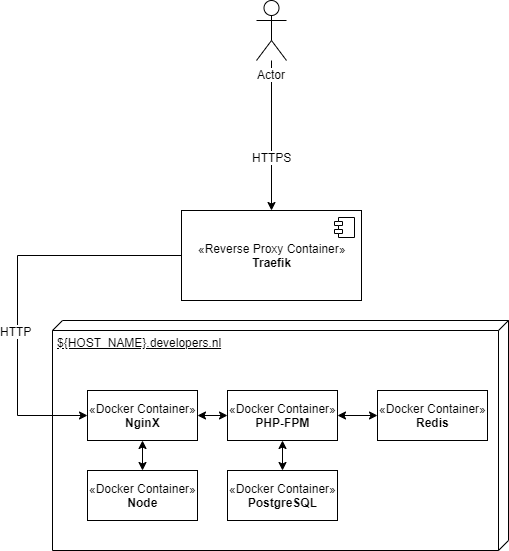
\includegraphics[width=13cm]{Figures/Traefik}
	\decoRule
	\caption[Traefik Infrastructure]{Nieuwe infrastructuur met Traefik reverse proxy}
	\label{fig:traefikinfrastructure}
\end{figure}
\begin{figure}[H]
	\centering
	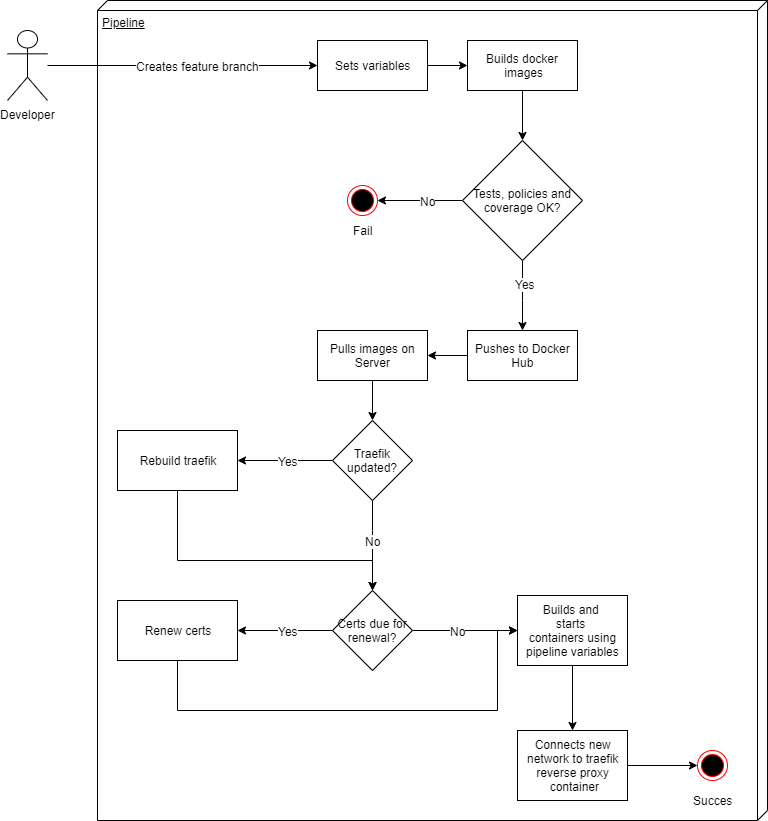
\includegraphics[width=13cm]{Figures/Activitydiagram}
	\decoRule
	\caption[Pipeline Activity Diagram]{Activity Diagram voor de pipeline}
	\label{fig:activitydiagram}
\end{figure}

docker/docker-compose.yml
\begin{minted}[linenos=true, bgcolor=codebg, breaklines]{yaml}
version: "3.4"

networks:
  nginx:
    driver: bridge

services:
  node:
    networks:
      - nginx
    environment:
      - NODE_ENV=production
      - BACKEND_URL=http://nginx:3000
    restart: always
    expose:
      - 3000

  nginx:
    restart: always
    networks:
      - nginx
    environment:
      - server_name=${server_name}
    labels:
      - traefik.enable=true
      - traefik.docker.network=${net_name}_nginx
      - traefik.http.routers.${net_name}_nginx.rule= Host(`${server_name}`) || Host(`werkenbij.${server_name}`)
      - traefik.http.routers.${net_name}_nginx.entrypoints=http
      - traefik.http.routers.${net_name}_nginx.middlewares= nginx-https-redirect
      - traefik.http.middlewares.nginx-https-redirect.redirectscheme. scheme=https
      - traefik.http.middlewares.nginx-https-redirect.redirectscheme. permanent=true
      - traefik.http.routers.${net_name}_nginx-secure.rule= Host(`${server_name}`) || Host(`werkenbij.${server_name}`)
      - traefik.http.routers.${net_name}_nginx-secure.entrypoints= https
      - traefik.http.routers.${net_name}_nginx-secure.tls=true
      - traefik.http.routers.${net_name}_nginx-secure.tls.options= myTLSOptions@file
    expose:
      - 8080
\end{minted}

docker/docker-compose.dev.yml
\begin{minted}[linenos=true, bgcolor=codebg, breaklines]{yaml}
version: "3.4"

volumes:
    development_ssl: ~

services:
  node:
    user: "1000"
    image: node:10.16.0-alpine
    volumes:
      - ../htdocs:/app:delegated
    environment:
      - NODE_ENV=development
    working_dir: /app
    command: ['/bin/sh', '-c', 'npm install --from-lock-file --no-optional --no-save && npm run dev']

  nginx:
    build:
      context: ./nginx 
      dockerfile: Dockerfile
    volumes:
      - development_ssl:/etc/letsencrypt/live/localhost
      - ./nginx/etc/nginx/temp/nginx.conf:/etc/nginx/temp/nginx.conf
      - ./nginx/etc/nginx/temp/conf.d:/etc/nginx/temp/conf.d
      - ../htdocs/static:/srv/html/static
    environment:
      - server_name=localhost
      - error_page=onderhoud.dev.html
      - php_backend_address=149.210.228.97:443
      - pass_type=proxy_pass https://phpbackend
      - cache_max_time=1s
      - hsts_max_time=0
      - cache_max_age=1
      - node_backend_address=node:3000
\end{minted}

docker/docker-compose.prod.yml
\begin{minted}[linenos=true, bgcolor=codebg, breaklines]{yaml}
version: "3.4"

volumes:
  logs: ~
  app_root: ~

services:
  node:
    image: "developersnl/node:${node_tag}"
    environment:
      - server_name=${server_name}

  nginx:
    image: "developersnl/nginx:${nginx_tag}"
    environment:
      - error_page=onderhoud.html
      - php_backend_address=php-fpm:9000
      - pass_type=fastcgi_pass phpbackend
      - php_app_location=/app/src/public
      - cache_max_time=4m
      - hsts_max_time=31536000
      - cache_max_age=31536000
      - node_backend_address=node:3000
    volumes:
      - /etc/developers.nl/static:/srv/html/static
      - logs:/var/log/nginx
\end{minted}

docker/docker-compose.proxy.yml
\begin{minted}[linenos=true, bgcolor=codebg, breaklines]{yaml}
version: "3.4"

volumes:
  development_ssl: ~

services:
  traefik:
    labels:
      - traefik.enable=true
      - traefik.http.routers.traefik.entrypoints=http
      - traefik.http.routers.traefik.rule=Host (`traefik.${root_server_name}`)
      - traefik.http.routers.traefik.middlewares= traefik-https-redirect
      - traefik.http.middlewares.traefik-https-redirect. redirectscheme.scheme=https
      - traefik.http.routers.traefik-secure.entrypoints=https
      - traefik.http.routers.traefik-secure.rule= Host(`traefik.${root_server_name}`)
      - traefik.http.routers.traefik-secure.middlewares=traefik-auth
      - traefik.http.routers.traefik-secure.tls=true
      - traefik.http.routers.traefik-secure.tls.options= myTLSOptions@file
      - traefik.http.routers.traefik-secure.service=api@internal
    environment:
      - TRAEFIK_PROVIDERS_DOCKER_EXPOSEDBYDEFAULT=false
      - TRAEFIK_PROVIDERS_FILE_FILENAME=/dynamic_conf.toml
      - TRAEFIK_API_INSECURE=false
\end{minted}

docker/docker-compose.proxy.prod.yml
\begin{minted}[linenos=true, bgcolor=codebg, breaklines]{yaml}
version: "3.4"

volumes:
  development_ssl: ~

services:
  traefik:
    image: developersnl/traefik:${traefik_tag}
    user: runuser
    ports:
      - 80:8080
      - 443:8443
    volumes:
      - /etc/traefik/dynamic_conf.toml:/dynamic_conf.toml
      - /etc/letsencrypt/live/${root_server_name}/fullchain.pem:/ssl/ fullchain.pem
      - /etc/letsencrypt/live/${root_server_name}/privkey.pem:/ssl/ privkey.pem
      - /home/runuser/.docker:/ssl/docker # TODO: runuser as variable
    labels:
      - traefik.http.middlewares.traefik-auth.basicauth.users= administrator:$$2y$$05$$WFGxILOwRePTQdqxrR8aoObKpf. ikMvpGv2ZLdEbRO13rmhuQo4xu
    environment:
      - TRAEFIK_ENTRYPOINTS_HTTP_ADDRESS=:8080
      - TRAEFIK_ENTRYPOINTS_HTTPS_ADDRESS=:8443
      - TRAEFIK_PROVIDERS_DOCKER_TLS_CAOPTIONAL=false
      - TRAEFIK_PROVIDERS_DOCKER_TLS_CA=/ssl/docker/ca.pem
      - TRAEFIK_PROVIDERS_DOCKER_TLS_CERT=/ssl/docker/cert.pem
      - TRAEFIK_PROVIDERS_DOCKER_TLS_KEY=/ssl/docker/key.pem
      - TRAEFIK_PROVIDERS_DOCKER_ENDPOINT=tcp://172.17.0.1:2376 # TODO BIP var
\end{minted}

docker/docker-compose.proxy.dev.yml
\begin{minted}[linenos=true, bgcolor=codebg, breaklines]{yaml}
version: "3.4"

volumes:
  development_ssl: ~

services:
  traefik:
    image: traefik:2.1
    ports:
      - 80:80
      - 443:443
    volumes:
      - ./traefik/dynamic_conf.toml/:/dynamic_conf.toml
      - /var/run/docker.sock:/var/run/docker.sock:ro
      - development_ssl:/ssl
    labels:
      - traefik.http.middlewares.traefik-auth.basicauth.users=test :$$apr1$$H6uskkkW$$IgXLP6ewTrSuBkTrqE8wj/ #test:test
    environment:
      - TRAEFIK_ENTRYPOINTS_HTTP_ADDRESS=:80
      - TRAEFIK_ENTRYPOINTS_HTTPS_ADDRESS=:443
      - TRAEFIK_LOG_LEVEL=debug
      - TRAEFIK_PROVIDERS_DOCKER_ENDPOINT=unix:///var/run/docker.sock

  ssl:
    build:
      context: ssl-dev
    volumes:
      - development_ssl:/ssl
\end{minted}
\begin{minted}[linenos=true, bgcolor=codebg, breaklines]{bash}
Makefile

SHELL := /bin/bash

MAKEFLAGS := --silent --no-print-directory

.DEFAULT_GOAL := help

.PHONY: help node.shell node.logs

export secrets_dir :=$(CURDIR)/../.devnl-backend-vault/
export root_server_name=localhost
export server_name=localhost
export net_name=localhost

help:
	@echo "Please use 'make <target>' where <target> is one of"
	@awk 'BEGIN {FS = ":.*?## "} /^[a-zA-Z0-9\._-]+:.*?## / {printf "\033[36m%-30s\033[0m %s\n", $$1, $$2}' $(MAKEFILE_LIST)

### Development commands ###

up: ## Up containers in development mode
	. ./docker/up.sh

down: ## Down containers in development mode
	docker-compose -f docker/docker-compose.yml -f docker/docker-compose.dev.yml -p ${server_name} down
	docker-compose -f docker/docker-compose.proxy.yml -f docker/docker-compose.proxy.dev.yml -p proxy down

restart: ## Restart containers in development mode
	docker-compose -f docker/docker-compose.yml -f docker/docker-compose.dev.yml -p ${server_name} restart
	docker-compose -f docker/docker-compose.proxy.yml -f docker/docker-compose.proxy.dev.yml -p proxy down

build: ## Build containers
	docker-compose -f docker/docker-compose.yml -f docker/docker-compose.dev.yml -p ${server_name} build
	docker-compose -f docker/docker-compose.proxy.yml -f docker/docker-compose.proxy.dev.yml -p proxy down

loadtest: ## Start influxdb + grafana on localhost:3000 and run a k6 load test
	docker-compose -f docker/docker-compose.k6.yml -p website up -d influxdb grafana
	docker-compose -f docker/docker-compose.k6.yml -p website run --rm k6 run /k6/test.js
	@echo Success! Grafana is running on http://localhost:3000
	@echo You should import a preconfigured dashboard like "https://grafana.com/grafana/dashboards/2587"

secrets.edit: ## Edit the vault file to remove or add secrets
	ansible-vault edit ansible/shared_vars/vault.yml --vault-password-file=../.vault-password

ansible.lint: ## Run Ansible Lint
	docker run \
		--rm \
		--workdir=/ansible \
		-v $(CURDIR)/ansible:/ansible \
		-it survivorbat/ansible:v0.3 \
		ansible-lint /ansible/site.yml

#stack:
#	POSTGRES_PORT=5432 \
#	docker stack deploy -c docker/docker-compose.swarm.yml --with-registry-auth website

### Node commands ###

node.shell: ## Enter the shell of the node container
	docker-compose -f docker/docker-compose.yml -f docker/docker-compose.dev.yml -p ${server_name} run --rm node sh

node.logs: ## See logs of the node container
	docker-compose -f docker/docker-compose.yml -f docker/docker-compose.dev.yml -p ${server_name} logs -f node

node.tests: ## Run tests in the node container
	docker-compose -f docker/docker-compose.yml -f docker/docker-compose.dev.yml -p ${server_name} run --rm node npm run test /app

storybook.run: ## Run storybook on port 6006
	docker run --rm -u node --name ${net_name}_storybook_1 -v ${CURDIR}/htdocs:/app --workdir=/app -p 6006:6006 node:10.16.0-alpine npm run storybook
	@echo Success! Storybook is now running over at http://localhost:6006

### e2e commands ###

# TODO: Make sure this does not run as root (setting the user makes it crash)
cypress.run: ## Run Cypress frontend tests locally against running containers
	docker run --rm \
	--network ${server_name}_nginx \
	--name ${server_name}_cypress_1 \
	-e CYPRESS_baseUrl=https://nginx:8443 \
	-v $(CURDIR)/e2e:/e2e \
	--workdir=/e2e \
	cypress/included:3.2.0 cypress run --spec "cypress/integration/frontend/**/*"

cypress.run.be: # Run Cypress backend test on the testserver (make sure you set the correct admin credentials in the command and to NOT commit them)
	docker run --rm \
	--network ${server_name}_nginx \
	--name ${server_name}_cypress_1 \
	-e CYPRESS_baseUrl="https://test.developers.nl" \
	-e CYPRESS_admin_username="" \
	-e CYPRESS_admin_password="" \
	-v $(CURDIR)/e2e:/e2e \
	--workdir=/e2e \
	cypress/included:3.2.0 cypress run --spec "cypress/integration/backend/**/*"
\end{minted}

docker/up.sh
\begin{minted}[linenos=true, bgcolor=codebg, breaklines]{bash}
#!/bin/bash

docker-compose -f docker/docker-compose.yml -f docker/docker-compose.dev.yml -p ${server_name} up -d
docker-compose -f docker/docker-compose.proxy.yml -f docker/docker-compose.proxy.dev.yml -p proxy up -d ssl traefik

networks=$(docker network inspect -f '{{range .Containers}}{{.Name}}{{end}}' ${net_name}_nginx)

if [[ $networks != *"proxy_traefik"* ]]; then
  echo "Connecting ${net_name}_nginx to proxy_traefik_1..."
  docker network connect ${net_name}_nginx proxy_traefik_1
fi
\end{minted}

docker/traefik/Dockerfile
\begin{minted}[linenos=true, bgcolor=codebg, breaklines]{bash}
FROM traefik:2.1

ARG USER_ID
ARG GROUP_ID

RUN addgroup -g ${GROUP_ID} rungroup \
 && adduser -u ${USER_ID} -S -G rungroup runuser \
 && mkdir -p /ssl/docker \
 && chown -R ${USER_ID}:${GROUP_ID} /ssl
\end{minted}

docker/traefik/dynamic\_conf.toml
\begin{minted}[linenos=true, bgcolor=codebg, breaklines]{toml}
[tls]
  [[tls.certificates]]
    certFile = "/ssl/fullchain.pem"
    keyFile = "/ssl/privkey.pem"

[tls.options]
  [tls.options.default]
    minVersion = "VersionTLS12"

  [tls.options.myTLSOptions]
    minVersion = "VersionTLS13"
    cipherSuites = [
        "TLS_ECDHE_ECDSA_WITH_AES_256_GCM_SHA384",
        "TLS_ECDHE_RSA_WITH_AES_256_GCM_SHA384",
        "TLS_ECDHE_ECDSA_WITH_AES_128_GCM_SHA256",
        "TLS_ECDHE_RSA_WITH_AES_128_GCM_SHA256",
        "TLS_ECDHE_ECDSA_WITH_CHACHA20_POLY1305",
        "TLS_ECDHE_RSA_WITH_CHACHA20_POLY1305"
    ]
\end{minted}

Vagrantfile
\begin{minted}[linenos=true, bgcolor=codebg, breaklines]{ruby}
# -*- mode: ruby -*-
# vi: set ft=ruby :

VAGRANTFILE_API_VERSION = "2"

Vagrant.configure(VAGRANTFILE_API_VERSION) do |config|
  config.vm.box = "ubuntu/bionic64"
  config.vm.network :private_network, ip: "192.168.33.39"
  config.ssh.insert_key = false

  config.vm.hostname = "docker.test"
  config.vm.provider :virtualbox do |v|
    v.name = "docker.test"
    v.memory = 1024
    v.cpus = 2
    v.customize ["modifyvm", :id, "--natdnshostresolver1", "on"]
    v.customize ["modifyvm", :id, "--ioapic", "on"]
  end

  # Enable provisioning with Ansible.
  config.vm.provision "ansible" do |ansible|
    ansible.compatibility_mode = "2.0"
    ansible.extra_vars = {
        node_tag: "website-latest",
        nginx_tag: "website-latest",
        add_latest_tag: "false"
    }
    ansible.galaxy_role_file = "./ansible/requirements.yml"
    ansible.playbook = "./ansible/site.yml"
    ansible.vault_password_file = "../.vault-password"
  end
end
\end{minted}

secure-daemon/defaults/main.yml
\begin{minted}[linenos=true, bgcolor=codebg, breaklines]{yaml}
---
system_tmp: /tmp
country: NL
state: Zuid Holland
locality: Rotterdam
organization: Developers.nl
host: 127.0.0.1
email: info@developers.nl
common_name: "{{ host }}"
passphrase: "{{ docker_cert_passphrase }}"
subject_alt_name: DNS:localhost,IP:172.17.0.1,IP:127.0.0.1
ca_cipher: aes256

server_cert_path: /etc/docker
client_cert_path: "/home/{{ default_user }}/.docker"
temp_path: "{{ system_tmp }}/ansible-secure-deamon"
csr_form_file: "{{ temp_path }}/csr_form.txt"
extfile: "{{ temp_path }}/extfile.cnf"
\end{minted}

secure-daemon/tasks/generate\_client\_certs.yml
\begin{minted}[linenos=true, bgcolor=codebg, breaklines]{yaml}
- name: Generate OpenSSL private key with default values (4096 bits, RSA)
  openssl_privatekey:
    path: "{{ server_cert_path }}/key.pem"

- name: Generate an OpenSSL Certificate Signing Request
  openssl_csr:
    path: "{{ server_cert_path }}/client.csr"
    privatekey_path: "{{ server_cert_path }}/key.pem"
    common_name: client
    extended_key_usage:
      - clientAuth

- name: Generate OpenSSL certificate signed with your own CA certificate
  openssl_certificate:
    path: "{{ server_cert_path }}/cert.pem"
    csr_path: "{{ server_cert_path }}/client.csr"
    ownca_path: "{{ server_cert_path }}/ca.pem"
    ownca_privatekey_path: "{{ server_cert_path }}/ca-key.pem"
    ownca_privatekey_passphrase: "{{ passphrase }}"
    provider: ownca

- name: Ensure {{ client_cert_path }}
  file:
    state: directory
    path: "{{ client_cert_path }}"
    owner: "{{ default_user }}"
    group: "{{ default_group }}"


- name: Copy client certs
  copy:
    remote_src: yes
    src: "{{ server_cert_path }}/{{ item }}"
    dest: "{{ client_cert_path }}/."
    owner: "{{ default_user }}"
    group: "{{ default_group }}"
  loop:
    - ca.pem
    - cert.pem
    - key.pem

- name: Ensure file permissions for keys
  file:
    path: "{{ client_cert_path }}/key.pem"
    mode: 0400

- name: Ensure file permissions for certificates
  file:
    path: "{{ client_cert_path }}/{{ item }}"
    mode: 0444
  loop:
    - ca.pem
    - cert.pem
\end{minted}

secure-daemon/tasks/generate\_server\_certs.yml
\begin{minted}[linenos=true, bgcolor=codebg, breaklines]{yaml}
- name: Generate OpenSSL private key with default values (4096 bits, RSA)
  openssl_privatekey:
    path: "{{ server_cert_path }}/server-key.pem"

- name: Generate OpenSSL Certificate Signing Request
  openssl_csr:
    path: "{{ server_cert_path }}/server.csr"
    privatekey_path: "{{ server_cert_path }}/server-key.pem"
    subject:
      commonName: "{{ common_name }}"
    subject_alt_name: "{{ subject_alt_name }}"

- name: Generate OpenSSL certificate signed with your own CA certificate
  openssl_certificate:
    path: "{{ server_cert_path}}/server-cert.pem"
    csr_path: "{{ server_cert_path }}/server.csr"
    ownca_path: "{{ server_cert_path }}/ca.pem"
    ownca_privatekey_path: "{{ server_cert_path }}/ca-key.pem"
    ownca_privatekey_passphrase: "{{ passphrase }}"
    provider: ownca

- name: "Ensure the server cert path {{ server_cert_path }}"
  file:
    state: directory
    path: "{{ server_cert_path }}"

- name: Ensure file permissions for keys
  file:
    path: "{{ server_cert_path }}/server-key.pem"
    mode: 0400

- name: Ensure file permissions for certificates
  file:
    path: "{{ server_cert_path }}/{{ item }}"
    mode: 0444
  loop:
    - ca.pem
    - server-cert.pem
\end{minted}


secure-daemon/tasks/main.yml
\begin{minted}[linenos=true, bgcolor=codebg, breaklines]{yaml}
---
- name: Create docker directory
  file:
    state: directory
    path: /etc/docker
    owner: "{{ default_user }}"
    group: "{{ default_group }}"
    mode: '600'

- name: Deploy Docker daemon.json
  template:
    src: etc/docker/daemon.json.j2
    dest: /etc/docker/daemon.json
    owner: "{{ default_user }}"
    group: "{{ default_group }}"
    mode: '600'

- name: Create a tempdir
  file:
    state: directory
    path: "{{ temp_path }}"

- name: Generate OpenSSL private key with default values (4096 bits, RSA) and passphrase
  openssl_privatekey:
    path: "{{ server_cert_path }}/ca-key.pem"
    cipher: "{{ ca_cipher }}"
    passphrase: "{{ passphrase }}"

- name: Ensure ca-key.pem permissions
  file:
    path: "{{ server_cert_path }}/ca-key.pem"
    mode: 0400

- name: Generate ca certificate   
  command: "openssl req -new -x509 -days 365 -key {{ server_cert_path }}/ca-key.pem -sha256 -out {{ server_cert_path }}/ca.pem -passin pass:{{ passphrase }} -subj '/C={{ country }}/ST={{ state }}>/L={{ locality }}/O={{ organization }}/CN={{ common_name }}'"

- name: Ensure CA certificate permissions
  file:
    path: "{{ server_cert_path }}/ca.pem"
    mode: 0444

- name: Create/Renew server certs
  include: generate_server_certs.yml

- name: Create/Renew client certs
  include: generate_client_certs.yml

- name: Ensure docker.service.d directory
  file:
    state: directory
    path: /etc/systemd/system/docker.service.d
    owner: "{{ default_user }}"
    group: "{{ default_group }}"
    mode: '644'

- name: Override docker service
  template:
    src: etc/systemd/system/docker.service.d/override.conf.j2
    dest: /etc/systemd/system/docker.service.d/override.conf
    owner: "{{ default_user }}"
    group: "{{ default_group }}"
    mode: '644'

- name: Restart daemon
  command: "systemctl daemon-reload"

- name: Restart docker
  command: "systemctl restart docker"
\end{minted}


secure-daemon/templates/etc/docker/daemon.json.j2
\begin{minted}[linenos=true, bgcolor=codebg, breaklines]{JSON}
{
  "tlsverify": true,
  "tlscacert": "{{ server_cert_path }}/ca.pem",
  "tlscert": "{{ server_cert_path }}/server-cert.pem",
  "tlskey": "{{ server_cert_path }}/server-key.pem",
  "hosts": ["0.0.0.0:2376", "fd://"]
}
\end{minted}

secure-daemon/templates/etc/systemd/system/docker.service.d/override.conf.j2
\begin{minted}[linenos=true, bgcolor=codebg, breaklines]{text}
[Service]
  ExecStart=
  ExecStart=/usr/bin/dockerd --containerd=/run/containerd/containerd.sock
\end{minted}

ansible/group\_vars/all.yml
\begin{minted}[linenos=true, bgcolor=codebg, breaklines]{yaml}
default_groups:
  # First group is the default group
  - name: rungroup
    gid: 9000
  - name: developer
    gid: 50000

default_users:
  # First user is the default user
  - name: runuser
    uid: 9000
    system: yes
    group: 'rungroup'
  - name: developer
    uid: 50000
    group: 'developer'
    password: "{{ developer_password }}"
    authorized_key: "{{ developer_authorized_keys }}"

default_sudo_groups:
  - developer

default_user: "{{ default_users[0].name }}"
default_group: "{{ default_groups[0].name }}"

pip_install_packages:
  - name: setuptools
  - name: pyopenssl
    version: 16.2.0
  - name: certbot-dns-transip
  - name: docker
  - name: docker-compose
  - name: cryptography
    version: 2.1
docker_install_compose: yes
\end{minted}


ansible/roles/frontend-images/defaults/main.yml
\begin{minted}[linenos=true, bgcolor=codebg, breaklines]{yaml}
docker_images:
  - dockerfile: docker/node/Dockerfile
    path: ../
    name: developersnl/node
    tag: "{{ node_tag }}"
    buildargs:
      node_version: 10.16.0
  - dockerfile: Dockerfile
    path: ../docker/nginx
    name: developersnl/nginx
    tag: "{{ nginx_tag }}"
  - dockerfile: Dockerfile
    path: ../docker/traefik
    name: developersnl/traefik
    tag: "{{ traefik_tag }}"
    buildargs:
      USER_ID: 9000
      GROUP_ID: 9000

add_latest_tag: yes
publish_images: no
docker_username: ""
docker_password: ""
docker_email: ""
\end{minted}

ansible/roles/frontend/defaults/main.yml
\begin{minted}[linenos=true, bgcolor=codebg, breaklines]{yaml}
---
local_base_dir: ../../../..
project_dir: /srv/app/frontend
project_dir_files:
  - "{{ local_base_dir }}/docker/docker-compose.yml"
  - "{{ local_base_dir }}/docker/docker-compose.prod.yml"
  - "{{ local_base_dir }}/docker/docker-compose.proxy.yml"
  - "{{ local_base_dir }}/docker/docker-compose.proxy.prod.yml"

nginx_host_config_directory: /etc/developers.nl/nginx
nginx_config_files:
  - { src: "{{ local_base_dir }}/docker/nginx/nginx.conf", dest: "{{ nginx_host_config_directory }}" }
  - { src: "{{ local_base_dir }}/docker/nginx/conf.d", dest: "{{ nginx_host_config_directory }}" }

traefik_host_config_directory: /etc/traefik
traefik_config_files:
  - { src: "{{ local_base_dir }}/docker/traefik/dynamic_conf.toml", dest: "{{ traefik_host_config_directory }}/dynamic_conf.toml" }

nginx_host_letsencrypt_email: sentry@developers.nl
nginx_host_letsencrypt_post_hook: 'docker restart $(docker ps -q --filter="name=traefik")'
nginx_host_static_directory: /etc/developers.nl/
local_static_directory: "{{ local_base_dir }}/htdocs/static"

env: test

static_root_files:
  - { src: 'etc/developers.nl/static/robots.txt', dest: 'robots.txt' }
  - { src: 'etc/developers.nl/static/sitemap.xml', dest: 'sitemap.xml' }

image_delete_until_time: 4h
\end{minted}

ansible/roles/frontend/tasks/application.yml
\begin{minted}[linenos=true, bgcolor=codebg, breaklines]{yaml}
---
- name: "Ensure Docker login"
  docker_login:
    username: "{{ docker_username }}"
    email: "{{ docker_email }}"
    password: "{{ docker_password }}"

- name: "Clean {{ project_dir }}"
  file:
    state: absent
    path: "{{ project_dir }}"

- name: "Ensure {{ project_dir }}"
  file:
    state: directory
    path: "{{ project_dir }}"
    owner: "{{ default_user }}"
    group: "{{ default_group }}"
    recurse: yes

- name: "Ensure files in {{ project_dir }}"
  copy:
    src: "{{ item }}"
    dest: "{{ project_dir }}/"
    owner: "{{ default_user }}"
    group: "{{ default_group }}"
  loop: "{{ project_dir_files }}"

- name: "Ensure static files in {{ nginx_host_static_directory }}"
  copy:
    src: "{{ local_static_directory }}"
    dest: "{{ nginx_host_static_directory }}"
    owner: "{{ default_user }}"
    group: "{{ default_group }}"

- name: "Ensure static root files in {{ nginx_host_static_directory }}"
  template:
    src: "{{ item.src }}"
    dest: "{{ nginx_host_static_directory }}/static/{{ item.dest }}"
    owner: "{{ default_user }}"
    group: "{{ default_group }}"
  loop: "{{ static_root_files }}"

- name: "Ensure {{ traefik_host_config_directory }}"
  file:
    state: directory
    path: "{{ traefik_host_config_directory }}"
    owner: "{{ default_user }}"
    group: "{{ default_group }}"
    recurse: yes

- name: "Ensure traefik files in {{ traefik_host_config_directory }}"
  copy:
    src: "{{ item.src }}"
    dest: "{{ item.dest }}"
    owner: "{{ default_user }}"
    group: "{{ default_group }}"
  loop: "{{ traefik_config_files }}"

- name: "Get BITBUCKET_BRANCH"
  set_fact:
    branch: "{{ lookup('env','BITBUCKET_BRANCH') }}"

# Subdomain retrieved from bitbucket branch name. For example `WEB-123`
- name: "Set subdomain"
  shell: echo {{ branch }} | grep -o 'WEB-[0-9]\+'
  when: "'feature/WEB-' in branch"
  register: subdomain

# server_name will be the FQDN. For example: `WEB-123.developers.nl`.
- name: "Set server name"
  set_fact:
    server_name: "{{ inventory_hostname if subdomain.stdout is undefined else subdomain.stdout + '.' + inventory_hostname}}"

# Net name is a stripped and cased-down server_name. For example: `web-123developersnl`
- name: "Get Net name"
  shell: echo {{ server_name }} | tr -dc '[:alnum:]_-' | tr '[:upper:]' '[:lower:]'
  register: net_name

- name: "Ensure stop old docker containers"
  docker_container:
    name: "{{ item }}"
    state: stopped
  loop:
    - website_node_1
    - website_nginx_1

- name: "Ensure Docker restart project {{ server_name }}"
  environment:
    node_tag: "{{ node_tag }}"
    nginx_tag: "{{ nginx_tag }}"
    server_name: "{{ server_name }}"
    net_name: "{{ net_name.stdout }}"
  docker_compose:
    state: present
    restarted: yes
    project_name: "{{ server_name }}"
    project_src: "{{ project_dir }}"
    files:
      - "docker-compose.yml"
      - "docker-compose.prod.yml"

- name: "Ensure Docker restart proxy"
  environment:
    traefik_tag: "{{ traefik_tag }}"
    root_server_name: "{{ inventory_hostname }}"
    server_name: "{{ server_name }}"
    net_name: "{{ net_name.stdout }}"
  docker_compose:
    state: present
    restarted: yes
    project_name: "proxy"
    project_src: "{{ project_dir }}"
    files:
      - "docker-compose.proxy.yml"
      - "docker-compose.proxy.prod.yml"
  when: bootstrap_proxy | bool

- name: "Connect {{ net_name.stdout }}_nginx to traefik"
  docker_network:
    name: "{{ net_name.stdout }}_nginx"
    connected:
      - proxy_traefik_1
    appends: yes

# There is option for network aliases in docker_network so we have to use shell
- name: "Connect {{ net_name.stdout }}_nginx to PHP-FPM"
  shell: "docker network connect --alias php-fpm {{ net_name.stdout }}_nginx websitebackend_php-fpm_1"
  ignore_errors: yes

- name: "Clean up images older than {{ image_delete_until_time }}"
  docker_prune:
    images: yes
    images_filters:
      dangling: false
      until: "{{ image_delete_until_time }}"
  register: prune_result

- debug:
    var: prune_result
\end{minted}

ansible/roles/frontend/tasks/letsencrypt.yml
\begin{minted}[linenos=true, bgcolor=codebg, breaklines]{yaml}
---
- name: "Ensure transip.ini"
  template:
    src: etc/letsencrypt/transip.ini.j2
    dest: /etc/letsencrypt/transip.ini
    owner: root
    group: root
    mode: '600'

- name: "Ensure TransIP key"
  copy:
    content: "{{ transip_key }}"
    dest: "/root/transip.key"
    owner: root
    group: root
    mode: '600'

- name: "Run certbot challenge"
  command: "certbot certonly
        --agree-tos
        -m {{ nginx_host_letsencrypt_email }}
        -d {{ inventory_hostname }}
        -d *.{{ inventory_hostname }}
        -a certbot-dns-transip:dns-transip
        --certbot-dns-transip:dns-transip-credentials /etc/letsencrypt/transip.ini
        --certbot-dns-transip:dns-transip-propagation-seconds 240
        --expand
        -n"

- name: "Ensure certbot-renewal.timer templates"
  template:
    src: "{{ item }}"
    dest: "/etc/systemd/system/"
    owner: root
    group: root
    mode: '644'
  loop:
    - etc/systemd/system/certbot-renewal.service
    - etc/systemd/system/certbot-renewal.timer

- name: "Start and enable service certbot-renewal.timer"
  service:
    name: "certbot-renewal.timer"
    state: started
    enabled: yes

- name: "Ensure dhparam.pem"
  openssl_dhparam:
    path: "/etc/letsencrypt/live/{{ inventory_hostname }}/dhparam.pem"
    owner: "{{ default_user }}"
    group: "{{ default_group }}"
    size: 2048

- name: "Ensure letsencrypt directory permissions"
  file:
    state: directory
    path: /etc/letsencrypt/live
    recurse: yes
    owner: "{{ default_user }}"
    group: "{{ default_group }}"
\end{minted}

ansible/site.yml
\begin{minted}[linenos=true, bgcolor=codebg, breaklines]{yaml}
---
- name: Ensure common
  hosts: all
  become: yes
  tags: server_install
  gather_facts: no
  vars_files:
    - shared_vars/vault.yml
  pre_tasks:
    - name: "Ensure python"
      raw: test -e /usr/bin/python || (apt -y update && apt install -y python-minimal)
      register: output
      changed_when: (output.stdout | length) > 0
  roles:
    - common

- name: Ensure secure TLS docker socket
  hosts: all
  become: yes
  gather_facts: true
  vars_files:
    - shared_vars/vault.yml
  roles:
    - { tags: server_install, role: geerlingguy.pip }
    - { tags: server_install, role: geerlingguy.docker }
    - { tags: server_install, role: secure-daemon }

# Ensure built images for the pipeline
- name: Ensure frontend images
  hosts: localhost
  connection: local
  vars_files:
    - shared_vars/vault.yml
  roles:
    - { tags: build_images,publish_images, role: frontend-images }

# Ensure frontend host
- name: Ensure Frontend
  hosts: frontend
  become: yes
  vars_files:
    - shared_vars/vault.yml
  roles:
    - { tags: server_install, role: geerlingguy.certbot }
    - { tags: server_deploy, server_install, role: frontend }
\end{minted}

docker/nginx/etc/nginx/temp/conf.d/0004\_developers.nl.conf
\begin{minted}[linenos=true, bgcolor=codebg, breaklines]{text}
server {
    listen 8080;

    server_name ${server_name} nginx;

    rewrite ^/(?!(?!admin).)*/$ /$1 permanent;
    port_in_redirect off;

    root /srv/html/static;

    location ~ ^/(api|admin|login|logout) {
        try_files $uri $uri/ @php;

        limit_req zone=req_limit_per_ip burst=90 nodelay;
        limit_conn conn_limit_per_ip 40;
    }
    
    location /werkenbij {
        return 301 https://werkenbij.${server_name};
    }
    
    location /sleutel {
    	default_type "text/html";
    	alias /srv/html/static/sleutel.html;
	}

    location ~ ^/(uploads|css|bundles|img) {
        try_files $uri $uri/ @php;

        add_header Cache-Control "public,max-age=${cache_max_age},immutable" always;

        limit_req zone=req_limit_per_ip burst=130 nodelay;
        limit_conn conn_limit_per_ip 45;
    }

    location /service-worker.js {
        add_header Cache-Control no-cache;
        expires 0;

        proxy_pass http://nodebackend;
        proxy_set_header X-Real-IP $remote_addr;
        proxy_set_header X-Forwarded-For $proxy_add_x_forwarded_for;
        proxy_set_header Host $http_host;
        proxy_set_header X-Forwarded-Proto $scheme;
        proxy_hide_header X-Powered-By;

        limit_req zone=req_limit_per_ip burst=40 nodelay;
        limit_conn conn_limit_per_ip 15;
    }

    location @php {
        ${pass_type};

        # PHP
        include fastcgi_params;
        fastcgi_param SCRIPT_FILENAME ${php_app_location}/index.php;

        # External proxy
        proxy_set_header X-Forwarded-For $proxy_add_x_forwarded_for;
        proxy_set_header X-Forwarded-Proto $scheme;
        proxy_set_header Host $http_host;
        proxy_set_header X-Real-IP $remote_addr;
        proxy_hide_header X-Powered-By;

        add_header Access-Control-Allow-Origin *;
        add_header 'Access-Control-Allow-Methods' 'GET, HEAD, OPTIONS, POST';

        limit_req zone=req_limit_per_ip burst=30 nodelay;
        limit_conn conn_limit_per_ip 15;
    }

    location @node {
        proxy_pass http://nodebackend;
        proxy_set_header X-Real-IP $remote_addr;
        proxy_hide_header X-Powered-By;
        proxy_cache DEVELOPERSNL_node;
        proxy_set_header X-Forwarded-For $proxy_add_x_forwarded_for;
        proxy_set_header Host $http_host;
        proxy_set_header X-Forwarded-Proto $scheme;

        limit_req zone=req_limit_per_ip burst=30 nodelay;
        limit_conn conn_limit_per_ip 15;
    }

    location / {
        try_files $uri $backendpool;
    }

    location ~ ^/_next/static/*. {
        proxy_pass http://nodebackend;
        proxy_set_header X-Real-IP $remote_addr;
        proxy_set_header X-Forwarded-For $proxy_add_x_forwarded_for;
        proxy_set_header Host $http_host;
        proxy_set_header X-Forwarded-Proto $scheme;
        proxy_hide_header X-Powered-By;
        proxy_hide_header Cache-Control;

        add_header Cache-Control "public,max-age=${cache_max_age},immutable" always;

        limit_req zone=req_limit_per_ip burst=80 nodelay;
        limit_conn conn_limit_per_ip 50;
    }

    error_page 500 502 503 504 /${error_page};
    location /onderhoud {
       root /srv/html/static;
       internal;
    }
}
\end{minted}

docker/nginx/etc/nginx/temp/conf.d/0004\_werkenbij.developers.nl.conf
\begin{minted}[linenos=true, bgcolor=codebg, breaklines]{text}
server {
    listen 8080;

    server_name werkenbij.${server_name};

    rewrite ^/werkenbij/(.*)/$ /$1 permanent;
    port_in_redirect off;

    root /srv/html/static;

    location / {
        try_files $uri /werkenbij$request_uri;
    }

    location ~ ^/(uploads|css|bundles|img) {
        try_files $uri $uri/ @backend;

        add_header Cache-Control "public,max-age=${cache_max_age},immutable" always;

        limit_req zone=req_limit_per_ip burst=130 nodelay;
        limit_conn conn_limit_per_ip 45;
    }

    location @backend {
        ${pass_type};

        # External proxy
        proxy_set_header X-Forwarded-For $proxy_add_x_forwarded_for;
        proxy_set_header X-Forwarded-Proto $scheme;
        proxy_set_header Host $http_host;
        proxy_set_header X-Real-IP $remote_addr;

        limit_req zone=req_limit_per_ip burst=30 nodelay;
        limit_conn conn_limit_per_ip 15;
    }

    location /robots.txt {
        alias /srv/html/static/block/robots.txt;
    }

    location /werkenbij {
        proxy_pass http://nodebackend;
        proxy_set_header X-Real-IP $remote_addr;
        proxy_hide_header X-Powered-By;
        proxy_cache DEVELOPERSNL_node;
        proxy_set_header X-Forwarded-For $proxy_add_x_forwarded_for;
        proxy_set_header Host $http_host;
        proxy_set_header X-Forwarded-Proto $scheme;

        limit_req zone=req_limit_per_ip burst=30 nodelay;
        limit_conn conn_limit_per_ip 15;

        internal;
    }

    location ~ ^/(_next|static) {
        proxy_pass http://nodebackend;
        proxy_set_header X-Real-IP $remote_addr;
        proxy_set_header X-Forwarded-For $proxy_add_x_forwarded_for;
        proxy_set_header Host $http_host;
        proxy_set_header X-Forwarded-Proto $scheme;
        proxy_hide_header X-Powered-By;
        proxy_hide_header Cache-Control;

        add_header Cache-Control "public,max-age=${cache_max_age},immutable" always;

        limit_req zone=req_limit_per_ip burst=40 nodelay;
        limit_conn conn_limit_per_ip 15;
    }

    error_page 500 502 503 504 /${error_page};
    location /onderhoud {
       root /srv/html/static;
       internal;
    }
}
\end{minted}

docker/ssl-dev/Dockerfile
\begin{minted}[linenos=true, bgcolor=codebg, breaklines]{bash}
# Docker image to generate SSL certificates for a root domain and a wildcard subdomain in your development environment
FROM alpine:latest

RUN apk update --no-cache \
 && apk add --no-cache openssl bash

WORKDIR /ssl

RUN ["/bin/bash", "-c", "openssl req \
                         -x509 \
                         -nodes \
                         -newkey \
                         rsa:4096 \
                         -keyout /ssl/privkey.pem \
                         -out /ssl/fullchain.crt \
                         -days 9999 \
                         -subj '/C=NL/ST=Zuid Holland/L=Rotterdam/O=Developers.nl/OU=Development/CN=*.localhost /emailAddress=info@developers.nl' \
                         -extensions san \
                         -config <( \
                           echo '[req]'; \
                           echo 'distinguished_name=req'; \
                           echo '[san]'; \
                           echo 'subjectAltName=DNS:localhost') \
                         && openssl x509 -in /ssl/fullchain.crt -out /ssl/fullchain.pem -outform PEM"]

ENTRYPOINT ["openssl"]
\end{minted}

Bitbucket-Pipelines.yml
\begin{minted}[linenos=true, bgcolor=codebg, breaklines]{yaml}
pipelines:
  default:
    - step:
        name: 'Build'
        image: survivorbat/ansible:v0.3
        caches:
          - docker
        script:
          - 'echo -e $VAULT_PASSWORD > ../.vault-password'
          - 'ansible-galaxy install -r ansible/requirements.yml'
          - 'ansible-playbook
            -e node_tag=website-latest
            -e nginx_tag=website-latest
            -e traefik_tag=website-latest
            -i ansible/inventories/local.yml
            --vault-password-file=../.vault-password
            -e add_latest_tag=false
            --tags=build_images ansible/site.yml'

  custom:
    e2e@test.developers.nl:
      - step:
          name: 'E2E @test.developers.nl'
          image: cypress/included:3.2.0
          caches:
            - node
          artifacts:
            - e2e/cypress/screenshots/**/*
          script:
            - 'cd e2e && CYPRESS_baseUrl=https://test.developers.nl cypress run'
    e2e@developers.nl:
      - step:
          name: 'E2E @developers.nl'
          image: cypress/included:3.2.0
          caches:
            - node
          artifacts:
            - e2e/cypress/screenshots/**/*
          script:
            - 'cd e2e && CYPRESS_baseUrl=https://developers.nl cypress run'
    deploy@test.developers.nl:
      - step:
          name: 'Deploy @test.developers.nl'
          deployment: test
          image: survivorbat/ansible:v0.3
          caches:
            - docker
          script:
            - 'echo -e $VAULT_PASSWORD > ../.vault-password'
            - 'ansible-galaxy install -r ansible/requirements.yml'
            - 'ansible-playbook
              -e node_tag=test-website-$BITBUCKET_BUILD_NUMBER
              -e nginx_tag=test-website-$BITBUCKET_BUILD_NUMBER
              -e traefik_tag=test-website-$BITBUCKET_BUILD_NUBER
              -e publish_images=true
              -e bootstrap_proxy=false
              --vault-password-file=../.vault-password
              -i ansible/inventories/test.yml
              --skip-tags server_install
              ansible/site.yml'
      - step:
          name: 'E2E @test.developers.nl'
          image: cypress/included:3.2.0
          caches:
            - node
          artifacts:
            - e2e/cypress/screenshots/**/*
          script:
            - 'cd e2e && CYPRESS_baseUrl=https://test.developers.nl cypress run'
    deploy@developers.nl:
      - step:
          name: 'Deploy @developers.nl'
          deployment: production
          image: survivorbat/ansible:v0.3
          caches:
            - docker
          script:
            - 'echo -e $VAULT_PASSWORD > ../.vault-password'
            - 'ansible-galaxy install -r ansible/requirements.yml'
            - 'ansible-playbook
              -e node_tag=website-$BITBUCKET_BUILD_NUMBER
              -e nginx_tag=website-$BITBUCKET_BUILD_NUMBER
              -e traefik_tag=website-$BITBUCKET_BUILD_NUMBER
              -e publish_images=true
              -e bootstrap_proxy=false
              --vault-password-file=../.vault-password
              -i ansible/inventories/production.yml
              --skip-tags server_install
              ansible/site.yml'
      - step:
          name: 'E2E @developers.nl'
          image: cypress/included:3.2.0
          caches:
            - node
          artifacts:
            - e2e/cypress/screenshots/**/*
          script:
            - 'cd e2e && CYPRESS_baseUrl=https://developers.nl cypress run'
    bootstrap@test.developers.nl:
      - step:
          name: 'Bootstrap @test.developers.nl'
          deployment: test
          image: survivorbat/ansible:v0.3
          caches:
            - docker
          script:
            - 'echo -e $VAULT_PASSWORD > ../.vault-password'
            - 'ansible-galaxy install -r ansible/requirements.yml'
            - 'ansible-playbook
              -e node_tag=test-website-$BITBUCKET_BUILD_NUMBER
              -e nginx_tag=test-website-$BITBUCKET_BUILD_NUMBER
              -e traefik_tag=test-website-$BITBUCKET_BUILD_NUMBER
              -e publish_images=true
              -e bootstrap_proxy=true
              --vault-password-file=../.vault-password
              -i ansible/inventories/test.yml
              ansible/site.yml'
    bootstrap@developers.nl:
      - step:
          name: 'Bootstrap @developers.nl'
          deployment: production
          image: survivorbat/ansible:v0.3
          caches:
            - docker
          script:
            - 'echo -e $VAULT_PASSWORD > ../.vault-password'
            - 'ansible-galaxy install -r ansible/requirements.yml'
            - 'ansible-playbook
                -e node_tag=website-$BITBUCKET_BUILD_NUMBER
                -e nginx_tag=website-$BITBUCKET_BUILD_NUMBER
                -e traefik_tag=website-$BITBUCKET_BUILD_NUMBER
                -e publish_images=true
                -e bootstrap_proxy=true
                --vault-password-file=../.vault-password
                -i ansible/inventories/production.yml
                ansible/site.yml'
options:
  docker: true

definitions:
  services:
    docker:
      memory: 3072
\end{minted}